\documentclass[assd_tp2_main.tex]{subfiles}

\begin{document}

\section{Efectos de audio}

\subsection{Reverbebrador}

\subsubsection{Implementación de eco simple}

Se implemento un eco simple utilizando el sistema

\begin{equation}
	y(n)=x(n)+gx(n-M)
\end{equation}

Se muestran a continuación los resultados con una señal de prueba

\begin{figure}[H]	
	\centering
	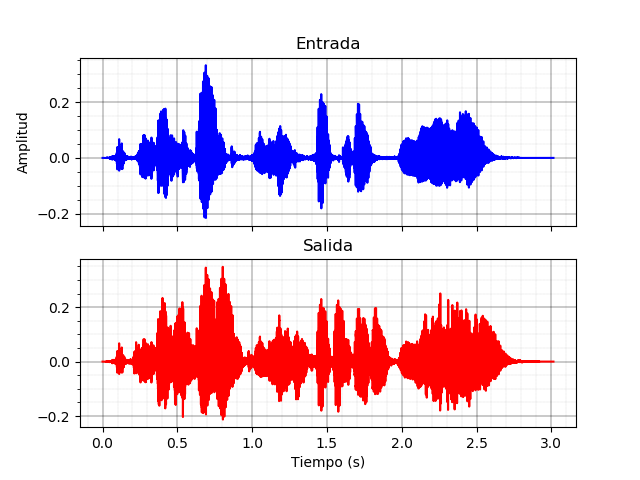
\includegraphics[scale=1]{graficos/EJ8/eco_simple.png}
	\caption{Resultados con $M=5000$, $g=0.999$ }
	\label{fig:bloqueElemental}
\end{figure}

Se puede observar de los resultados intuitivamente como la señal de salida contiene repeticiones de la señal de entrada, y al escuchar el audio se pudo notar dicho efecto de eco. Fue necesario colocar un retraso muy grande ($M=5000$) y una ganancia muy alta ($g=0.999$) para que el efecto fuera notorio

\subsubsection{Implementación de reverberación plana}
Se implementó una reverberación plana utilizando una ecuación de diferencias con feedback. 
\begin{equation}
	y(n)=x(n)+gy(n-M)
\end{equation}
Se muestran a continuación los resultados con una señal de prueba
\begin{figure}[H]	
	\centering
	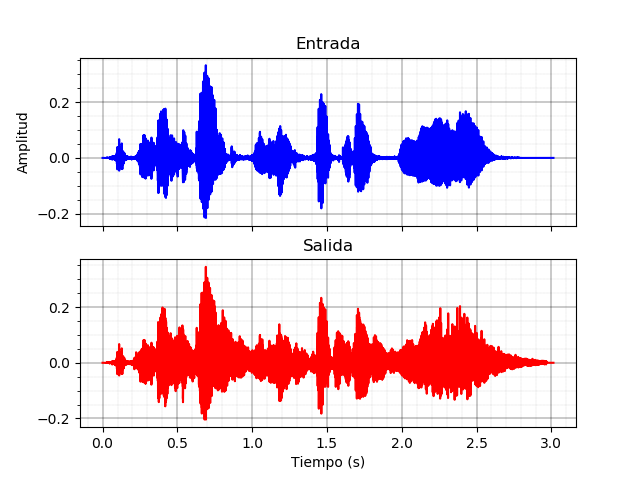
\includegraphics[scale=1]{graficos/EJ8/eco_plano.png}
	\caption{Resultados reverberación plana con $M=500$, $g=0.5$ }
	\label{fig:bloqueElemental}
\end{figure}
Se necesitó disminuir fuertemente el valor de $g$ para evitar que la salida saturara. Al tener realimentación (es decir, ser IIR) el sistema puede perder la estabilidad con facilidad

\subsubsection{Implementación de reverberación pasa bajos}

Se le agrego un filtro pasabajo a la realimentación del sistema anterior. Se optó por un sencillo pasabajos similar al utilizado en el modelo Karplus Strong, de la forma $y(n)=\frac{x(n)+x(n-1)}{2}$
El sistema por lo tanto quedo descrito como
\begin{equation}
y(n)=x(n)+\frac{1}{2}g(y(n-M)+y(n-M-1))
\end{equation}
\begin{figure}[H]	
	\centering
	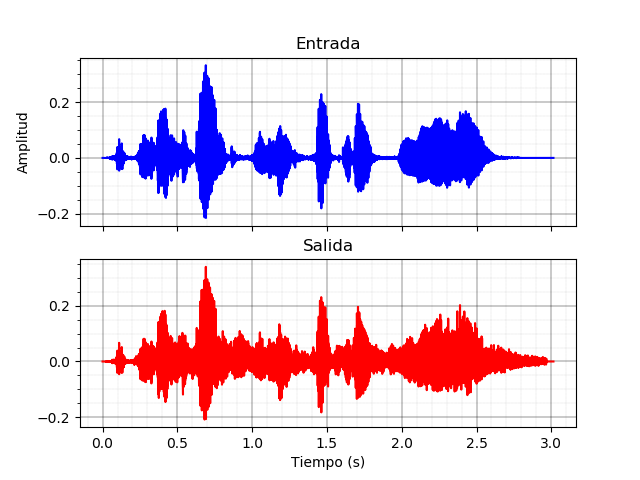
\includegraphics[scale=1]{graficos/EJ8/eco_pb.png}
	\caption{Resultados reververación con pasabajos $M=500$, $g=0.5$ }
	\label{fig:bloqueElemental}
\end{figure}

La señal fue similar al resultado del caso anterior con una sutil diferencia, el sonido se escuchó un con poco menos ruido, esto se debe muy probablamente a que el filtro pasa bajos evito la propagación de una frecuencia no deseada la cual no estaba presente en la señal original.

\subsubsection{Implementación de reverberación completa}

\subsubsection{Implementación de reverberación por convolución}
Se implemento una reverberación utilizando convolución con la respuesta al impulso característica de una fabrica. Se utilizo la ecuación de diferencias génerica siguiente

\begin{equation}
y(n)=\sum_{i=k}^{N}h(k)x(n-k)
\end{equation}

Debido a la complejidad algoritmica de la aplicación de la fórmula se debió limitar la longitud de la respuesta al impulso a solo 20000 muestras. Se muestran a continucación los resultados con una señal de prueba

\begin{figure}[H]	
	\centering
	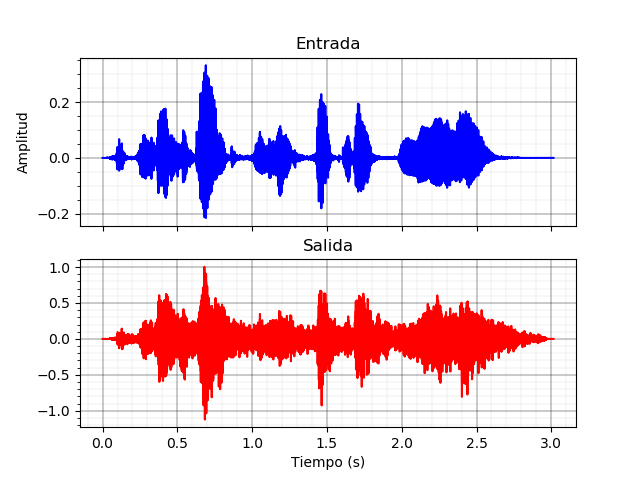
\includegraphics[scale=1]{graficos/EJ8/eco_convolucion.png}
	\caption{Resultados reverberación característica de una fábrica}
	\label{fig:bloqueElemental}
\end{figure}

Se observa como a diferencia de los casos anteriores la señal tiende mucho más a sostener sonido, esto se debe a que la respuesta al impulso es mucho más completa, y por lo tanto el sonido resultante persiste más tiempo.
El sonido que se escuchó se correspondió con un eco muy realista, que podría ser el de una fábrica

\end{document}

